Date: 15/08/2020

=-\chapter{Energy conservation between 2D motions}

% Date: 5/9/2020

\section{Aim}

In this experiment, our aim is to understand how energy is transferred when objects collide by varying the angle at which an object is released to collide with another.


\section{Background Theory}

 According to principle of physics energy is always conserved in a close system. Therefore, energy can be in different firms but the total energy remains the same. 
Energy for a moving object is kinetic energy and can be calculated using 
$$ E=\frac{1}{2} m v^2$$
and gravitational potential energy is when an object is stationary at a height and is has the ability to move. It is given by the equation $$E=mgh$$
For an object in projectile motion the position of body in x and y position are as following:
$$x(t) =x_0 +v_{0,x}t $$ 
$$y(t)= y_0 +v_{0,y}t -\frac {1}{2}gt^2$$
There is no acceleration in the horizontal direction, just a constant velocity but in the vertical direction there is constant acceleration. 
When two objects collide, the distance that the ball will reach the ground is 
$$d=2\sqrt{hL(1-\cos(\theta)}$$ where h denotes height pf collision, L is length of pendulum, $\theta$ is angle from which the swinging pendulum is placed. 

\section{Description of Setup}
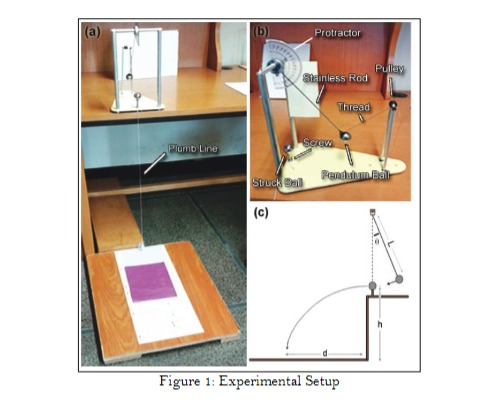
\includegraphics[width=10cm, height=7cm]{figures/figm.jpeg} \\
Here a pendulum is strung over a pulley with a fixed protractor and a metal ball is placed as shown in the figure. White sheets are placed below with a carbon paper on top to locate the position of the ball when released. A meter rule is also required.

\section{Method / Procedure}
The vertical height from the center of the ball to the ground is measured and marked. White papers are fixed to the ground with carbon paper on top. 
The pendulum is held at a high position at an angle of 30 measured through the fixed protractor on the pendulum and swung. It strikes the ball which follows a parabolic path and strikes the carbon sheet placed on the white papers on the floor. Repeat this process four times at the same angle. 
The same steps should be repeated at an angle of 40, 50 and 60 degrees and 5 readings should be taken at each angle. The length, d, of all the points of impact from initial position is measured and compared with theoretical predictions.  . 


\section{Data}

In this experiment, the constants h and L were only measured once and therefore don't have any Type A uncertainty. The type B uncertainty associated with both h and L is respectively  0.0002m. Consequently, $ h = 0.935 \pm 0.0002$m and $ L = 0.25 \pm 0.0002m $. The angle $\theta$ was also only measured only it doesn't have type A uncertainty. The type B associated with the angle $\theta $ is $ 0.04 $ degrees. The distance d was measured multiple and therefore it has both type B and type A uncertainty.
The recorded values for the angle $\theta$
\begin{center}
\begin{tabular}{|c|c|c|}
\hline
\textbf{s.No} & \textbf{Angle} & \textbf{angle (°)} \\ \hline
1             & A1             & 30                 \\ \hline
2             & A2             & 40                 \\ \hline
3             & A3             & 50                 \\ \hline
4             & A4             & 60                 \\ \hline
\end{tabular}
\end{center}

The values measured for the distance d (cm).
\begin{center}
\begin{tabular}{|l|l|l|l|l|}
\hline
\textbf{s.No} & \textbf{d\_A1 (cm)} & \textbf{d\_A2 (cm)} & \textbf{d\_A3 (cm)} & \textbf{d\_A4 (cm)} \\ \hline
1             & 30.5                & 42.7                & 55                  & 64.7                \\ \hline
2             & 31.5                & 43.3                & 55.7                & 63.8                \\ \hline
3             & 31.8                & 43                  & 57.7                & 65.4                \\ \hline
4             & 32.7                & 44.6                & 54                  & 65.3                \\ \hline
5             & 31.4                & 43.5                & 54.8                & 64.7                \\ \hline
\end{tabular}
\end{center}
Type A uncertainty in distance d when Angle($\theta = 30$)
\begin{center}
$\sigma_d = 0.0071m$ \\
$ U_d^A =  0.0035m$ \\
\end{center}
Type A uncertainty in distance d when Angle($\theta = 40$)
\begin{center}
$\sigma_d = 0.0065m$ \\
$ U_d^A =  0.0032m$ \\
\end{center}
Type A uncertainty in distance d when Angle($\theta = 50$)
\begin{center}
$\sigma_d = 0.0125m$ \\
$ U_d^A =  0.0063m$ \\
\end{center}
Type A uncertainty in distance d when Angle($\theta = 60$)
\begin{center}
$\sigma_d = 0.0057m$ \\
$ U_d^A =  0.0029m$ \\
\end{center}



\section{Data Analysis}
We will calculate the expected value for d using the following formula
    $$ d = 2 \sqrt{hL(1-cos(\theta))}$$
where h and L are constants with the values $ h = 0.935m$ and $L = 0.25m$\\

\begin{center}
\begin{tabular}{|l|l|l|}
\hline
s.No & Angle(°) & Expected value of d(m) \\ \hline
1    & 30       & 0.3539                 \\ \hline
2    & 40       & 0.4677                 \\ \hline
3    & 50       & 0.5779                 \\ \hline
4    & 60       & 0.6837                 \\ \hline
\end{tabular}
\end{center}

Average Value of the distance d for each value of the Angle($\theta$)
\begin{center}
\begin{tabular}{|l|l|l|l|}
\hline
s.No & Angle(°) & Avg\_d (cm) & Avg\_d(m) \\ \hline
1    & 30       & 31.58       & 0.316     \\ \hline
2    & 40       & 43.42       & 0.434     \\ \hline
3    & 50       & 55.44       & 0.554     \\ \hline
4    & 60       & 64.78       & 0.648     \\ \hline
\end{tabular}
\end{center}

\newpage
The graph of average distance d  vs Angle ($\theta$)
\begin{figure}[h!]
    \centering
    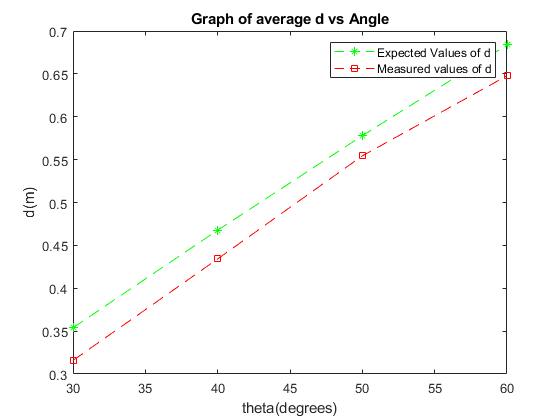
\includegraphics[width=\textwidth]{figures/Avg_d_vs_theta.png}
    \caption{Graph of Average d vs Angle ($\theta$)}
    \label{fig:yx}
\end{figure}
\newpage
Residual plot for d as when $\theta = 30 $
\begin{figure}[h!]
    \centering
    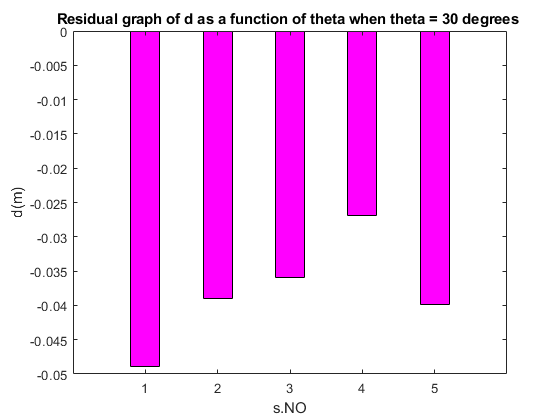
\includegraphics[width=\textwidth]{figures/d_A1_r.png}
    \caption{Residual Plot for  d when Angle ($\theta$ = 30)}
    \label{fig:yx}
\end{figure}
\newpage
Residual plot for d as when $\theta = 40 $
\begin{figure}[h!]
    \centering
    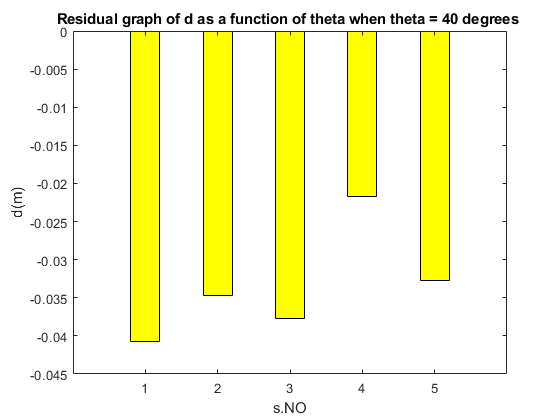
\includegraphics[width=\textwidth]{figures/d_A2_r.png}
    \caption{   Residual Plot for d when Angle($\theta$ = 40)}
    \label{fig:yx}
\end{figure}
\newpage 
Residual plot for d as when $\theta = 50 $
\begin{figure}[h!]
    \centering
    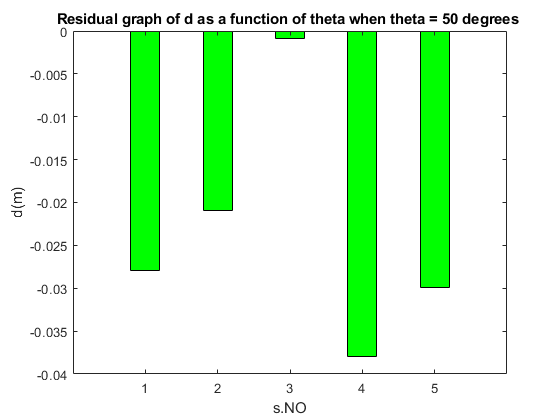
\includegraphics[width=\textwidth]{figures/d_A3_r.png}
    \caption{Residual Plot for  d when Angle ($\theta$ = 50)}
    \label{fig:yx}
\end{figure}
\newpage 
Residual plot for d as when $\theta = 60 $
\begin{figure}[h!]
    \centering
    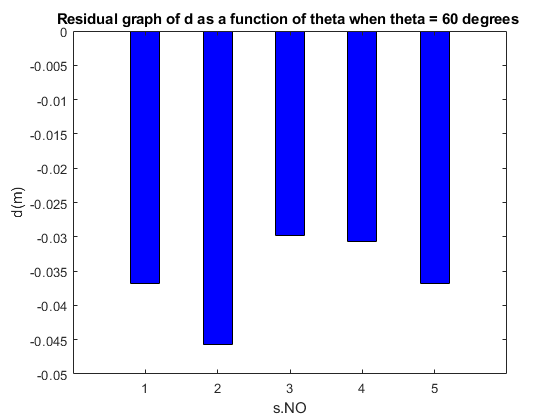
\includegraphics[width=\textwidth]{figures/d_A4_r.png}
    \caption{Residual Plot for d when Angle  ($\theta = 60$) }
    \label{fig:yx}
\end{figure}
We can transfer uncertainty from Angle($\theta$) to distance (d) using the following formula:
$$ U_d = \sqrt{{U_T^A}^2 +{U_T^B}^2+\biggr({\frac{\sqrt{hL}sin(\theta)\Delta\theta}{\sqrt{1-cos(\theta)}}}\biggr)^2}$$

\begin{center}
\begin{tabular}{|l|l|l|}
\hline
Expected value of   d(m) & Total Uncertainty in d(m) & Final Value(m)                     \\ \hline
0.316                    & 0.0272                     & $0.316 \pm 0.027$ \\ \hline
0.434                    & 0.0264                     & $ 0.434\pm 0.026$   \\ \hline
0.554                    & 0.0261                     & $ 0.554\pm 0.061$   \\ \hline
0.648                    & 0.0243                     & $ 0.648\pm 0.024$   \\ \hline
\end{tabular}
\end{center}
\newpage
\begin{figure}[h!]
    \centering
    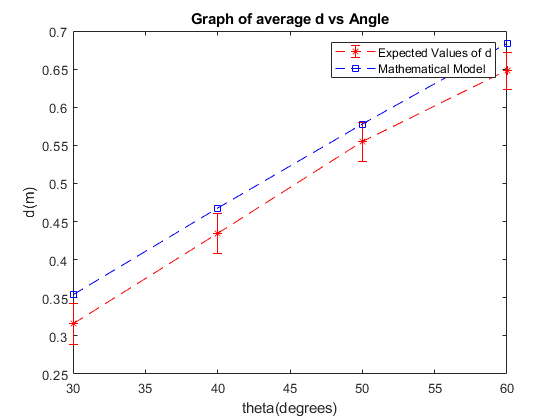
\includegraphics[width=\textwidth]{figures/Mathematical_Model.png}
    \caption{Graph of d vs Angle($\theta$)}
    \label{fig:yx}
\end{figure}


\section{Discussion \& Conclusion}
For our experiment and data, we can evaluate that at angle 30, theoretical value of d should be 0.3539 and our experimental value is 0.316 with error of 0.027. The theoretical value does not lie in the range $0.316 \pm 0.027$. Whereas for angle of 40, and 50 it does but not 60. We can also see that all our measured values are below expected values of d from figure 4.1. This implies that it is difficult to conclude if hypothesis is valid because half values agree with theoretical values. Possible factors of uncertainty could be wind and parallax errors in measuring the distances using metre rule. Air resistance could also cause experimental values to be less than the theoretical values since it acts as an opposing force. Furthermore, it may be difficult to locate exact location of where the ball may have struck first as it may touch several points on the carbon paper. A more accurate set up could have given results with the hypothesis that could include wind blockers, a camera or motion detector to ensure exact location of contact can be recorded. To deduce a better conclusion, the experiment should be carried out on multiple angles or in a setup to minimize air resistance so that a conclusion may be reached.     

% Summarize and discuss the experimental results, what do the results say about your hypothesis, if such a hypothesis was made for the experiment. Mention the uncertainty in the calculated quantity Be precise and only include scientific discussion.


\section{MATLAB Script}
\lstinputlisting{matlabCodes/Experiment4.m}

